
\section{Organizing DMA Risks}\label{sec:dma-risks}
In this section we organize and categorize the risks associated with DMA operations.
We first we categorise the different types of \subpage{} vulnerabilities.
Then, we categorize MMO, a trifecta of attributes, providing building blocks for reasoning about code-injection attacks.
These paint a clear picture of risks and dangers posed by DMA capable devices.
%We also discuss dangerous trade-offs and discuss the threat model.

\subsection{Sub-Page Vulnerability}\label{sec:subpage}

We classify the different types of potentially co-located data, into four categories, as illustrated in Fig.~\ref{fig:colocation}:

\begin{enumerate}
    \item[(a)] The I/O buffer is part of a bigger data structure. This data structure may include function pointers, often caused by poor DMA hygiene by the driver. An isolated driver fix is usually sufficient to fix such vulnerabilities.
    \item[(b)] The OS (e.g., memory allocator) rather than the driver saves metadata, such as free-lists, on the same page as the I/O buffer \cite{Cor07}. Manipulating these data structures may also compromise the system \cite{ak09}. Similarly to (a), sensitive metadata is unwittingly shared. However, in this case, it is an OS subsystem that is at fault rather than the device driver.
    \item[(c)] The same page is mapped multiple times due to co-located device driver buffers resulting in multiple \iova{} indicating the same page. 
    %A seemingly benign case, made dangerous by the fact that unmapping one \iova{} is meaningless, security-wise. 
    In this case, unmapping an \iova will not stop the device from accessing the page.
    That is, the device will retain access to the physical page as long as a single valid \iova{} exists.
    \item[(d)] The I/O buffer and a different, dynamically allocated memory buffer may coincidentally share a page. This common situation results in data leakage (e.g., kernel pointers). Currently, the Linux kernel uses the same memory allocation mechanism (e.g., kmalloc) for both I/O buffers and regular kernel buffers. Consequently, I/O buffers often share pages with other, potentially sensitive, kernel buffers. Since IOMMU works in page granularity, the respective I/O devices gain access to these kernel buffers as well. This is a subclass of (b), as an OS subsystem causes it, but the main difference is that the exposed data structures are leaked randomly.

\end{enumerate}

\begin{figure}[t]
    \centering
    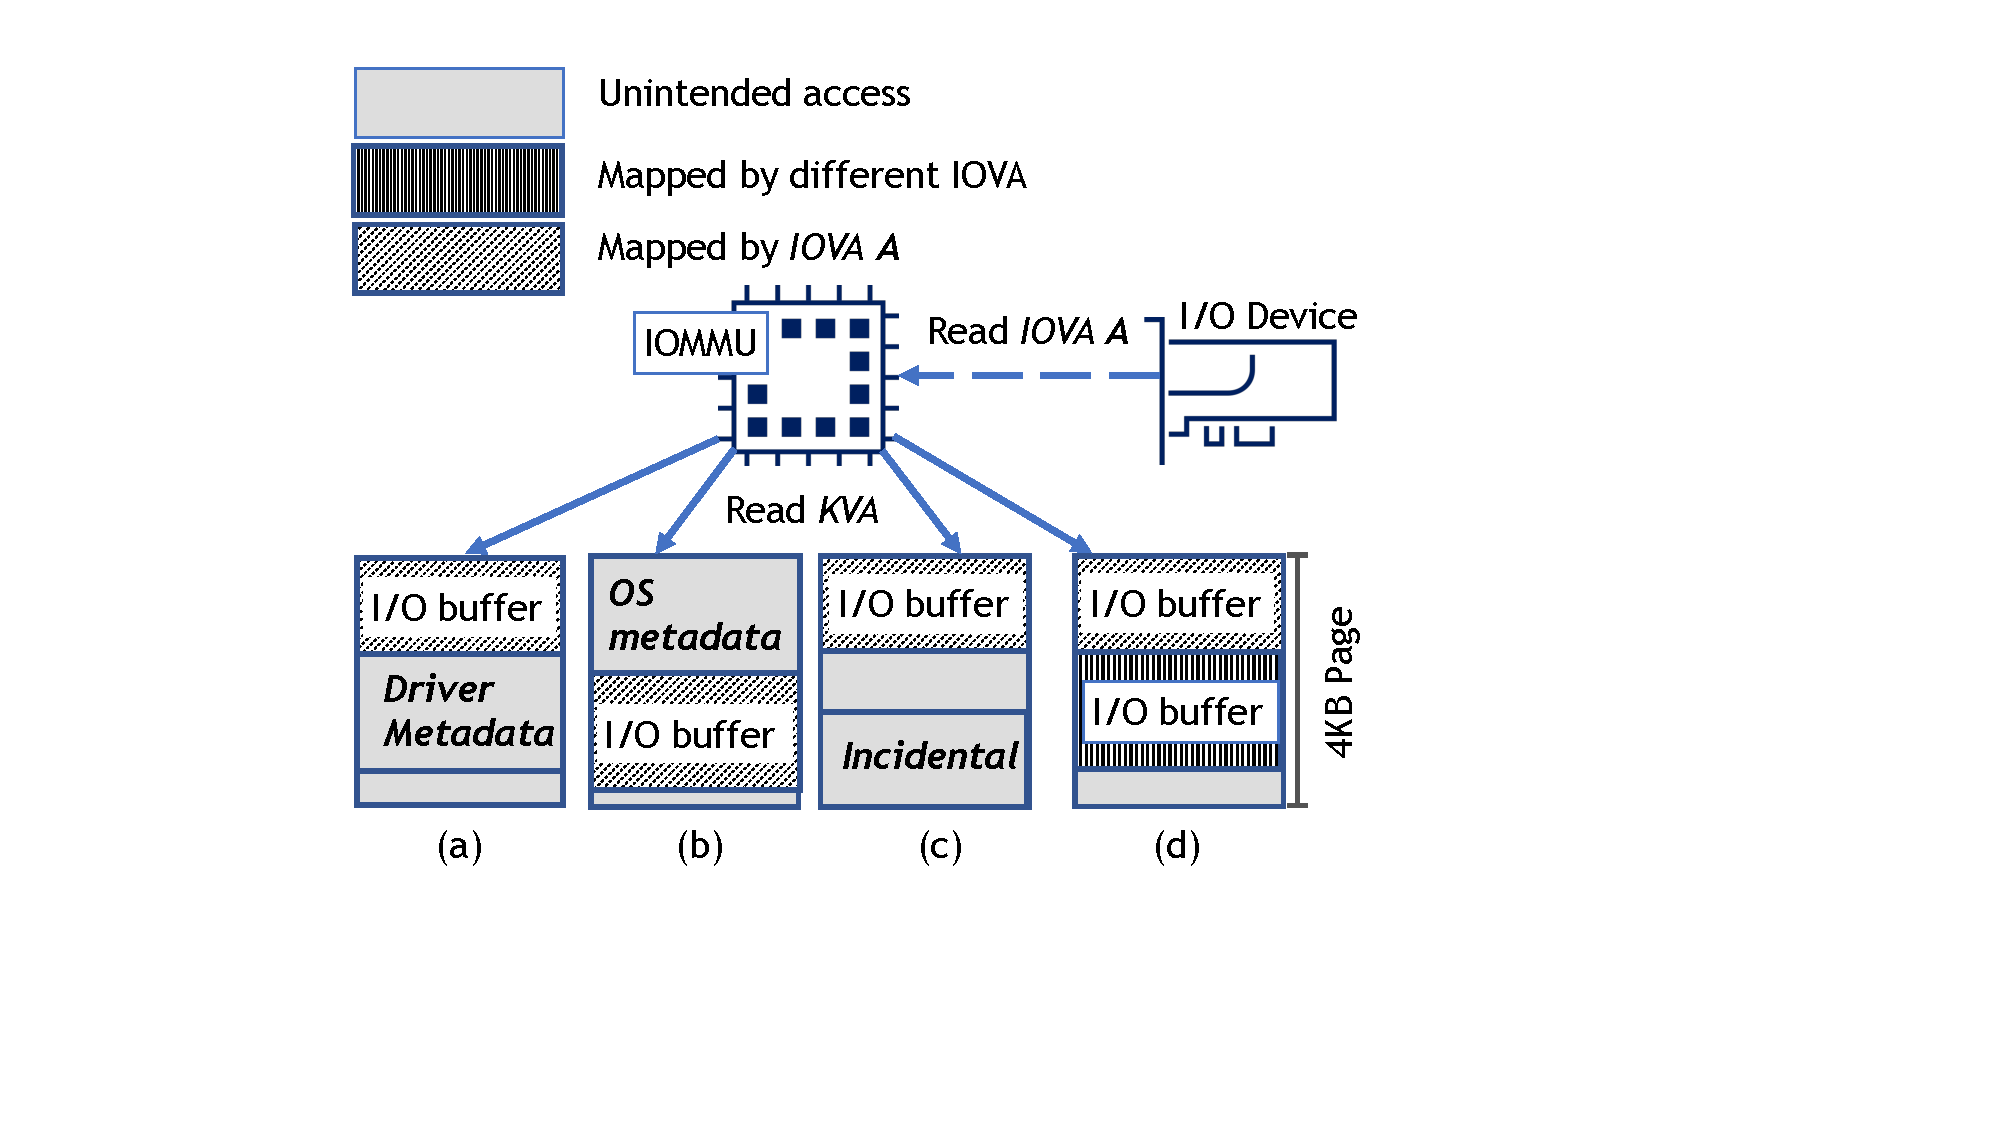
\includegraphics[width=0.9\columnwidth]{figs/subpage.pdf}
    \caption{\subpage{} DMA vulnerabilities when the I/O buffer shares a page with other data: (a) I/O buffer metadata; (b) OS
metadata; (c) a page mapped by multiple \iova; (d) randomly co-located sensitive buffers.}
    \label{fig:colocation}
\end{figure}


In the next sections we demonstrate how a \simple{} attack utilizes type (a) vulnerability (Sec. \ref{sec:sbp2_attack}). A \emph{compound attack}, on the other hand, uses type (b) and (c) vulnerabilities (Sec. \ref{sec:linux_net}). 
We also demonstrate the risks associated with type (d) vulnerability in Sec. \ref{sec:dma-kasan}. Type (d) vulnerability simplifies KASLR subversion~(\ref{sec:kaslr}) and opens viable attack vectors. 


\subsection{MMO}\label{sec:mmo}

We introduce the \motivation, \means, \oportunity (MMO) schema that allows for a systematic analysis of code-injection attacks by DMA capable devices.
%to categorizes DMA vulnerabilities. The goal of MMO is to define building blocks for reasoning about DMA attacks.
To execute a successful privilege escalation attack (i.e., code injection), a malicious device, just like a human criminal, needs Motive, Means, and Opportunity:
\begin{enumerate}
    \item \motivation: The \kva{} of a kernel buffer filled with malicious code (e.g., a ROP attack). Given the device is using \iova, the attacker needs to obtain the buffer's \kva{}, for example, by observing leaked pointers. 
    \item \means: Write access to a function callback pointer, which can alter the CPU control flow and cause it to execute the malicious code. For example, write access to a data structure that holds a function callback pointer, at a known offset.\footnote{The Linux kernel randomizes the layout of some data structures with \_\_randomize\_layout annotation \cite{rand_layout}.} The location on the page of the callback pointer must be known to the device.
    \item \oportunity: There exists a time window such that modifying \means during that time window is followed by the CPU reading the pointer without previously altering its content.
\end{enumerate}

To further emphasize the significance of the MMO attributes, we present a hypothetical scenario. Assume a NIC has write access to a page containing an RX packet (i.e., a received packet). Due to \subpage{} vulnerability and a random allocation coincidence (Fig. \ref{fig:colocation}, type (d)), a structure with a callback pointer is inadvertently accessible with write permission. Also, the malicious device is able to create a valid \mabaf{} in the aforementioned page. It may seem that the device has a valid attack, whereas it actually lacks MMO.

\begin{itemize}
    \item Missing \motivation: Without a valid \kva{} of the writable page, the device cannot modify the callback function pointer to indicate the \mabaf.
    \item Missing \means: Although a callback function pointer is available for modifications, the device has no way of knowing: 
    \begin{enumerate}
        \item[(a)] That a callback function pointer is available for sabotage.
        \item[(b)] The correct offset of the callback function pointer.
    \end{enumerate}
    \item Its not known if an \oportunity is actually available.
\end{itemize}

Under the hypothesized circumstance, and without additional information, a malicious device has practically no valid attack options. 
And while corrupting random kernel memory is still a possibility and may even cause a kernel panic \cite{MMT16}, it does not achieve the goal of privilege escalation.


%The MMO schema covers both random and deterministic attacks. 
%In this paper, we focus on demonstrating and addressing deterministic attacks, where the attacker is able to deduce the layout of the targeted data structure and its location on a page. 
%Random access attacks, also exploit the sup-page vulnerability and should not be taken lightly. Successful execution of random access attacks requires a more in-depth analysis to produce a viable chance of success. Accordingly, in Sec. \ref{sec:dma-kasan}, we present a run-time analysis tool capable of identifying such vulnerabilities. \adam{if there's a whole section about it, why the disclaimer that the paper focuses on deterministic attacks?}

\subsection{Extending MMO}
\textcolor{olive}{The MMO schema is especially useful for vulnerability analysis. For example, we show that a privilege escalation attack requires the full trifecta to be realized. Other high impact attacks, such as a full memory dump, may still be viable with only \oportunity{} given.}\adam{this paragraph can be dropped}

%KASLR is designed to stop code injection attacks. This indeed holds as long as kernel pointers are not leaked, an assumption that is not valid for DMA capable devices. For example, an OS leaks kernel pointers to a NIC, on pages containing small TX buffers. A malicious NIC can even spoof seemingly legitimate packets (e.g., ARP, ICMP, ICMPv6) to trigger kernel pointer leakage.

%Both attack types use type (d) vulnerability to compromise KASLR. KASLR is designed to stop code injection attacks. This indeed holds as long as kernel pointers are not leaked, an assumption that is not valid for DMA capable devices. For example, an OS leaks kernel pointers to a NIC, on pages containing small TX buffers. A malicious NIC can even spoof seemingly legitimate packets (e.g., ARP, ICMP, ICMPv6) to trigger kernel pointer leakage. \textcolor{olive}{We demonstrate the risks associated with type (d) vulnerability in Sec. \ref{fig:dkasan-report}.}


On the other hand, a full memory dump attack can be executed by merely having \oportunity.
%\adam{this looks weird. MMO can describe \emph{any} attack. For example, motive: read all memory; means: some kernel pointer; opportunity: the kernel pointer is DMA-writable}
That is, with \oportunity given, an attacker is able to modify the kernel control flow in such a way as to cause it to map arbitrary kernel addresses. For example, with write access to an I/O scatter-gather list a malicious device can control which memory pages are mapped to the device. This would result in a full memory dump.
%\adam{description isn't clear: it's modifying control-flow, so is it a code injection attack?} 
%In order to achieve this, an attacker needs to modify a kernel pointer once before it is mapped and, for a second time before send (i.e., TX) completion in order to avoid memory corruption (Sec. \ref{sec:linux_net}). 

%We demonstrate in Section \ref{sec:linux_net}, how an adversary can take advantage of \emph{deferred} mode.
